\documentclass[tikz,border=9pt,12pt]{standalone}
\usepackage{amsmath,amssymb}
\usetikzlibrary{arrows.meta,calc}
\tikzset{every node/.style={text=black,font=\normalsize},axis/.style={-{Stealth[length=2mm]},black!65,thin},vec/.style={-{Stealth[length=2.8mm]},line width=1.3pt,blue!70!black},lab/.style={fill=white,inner sep=2pt}}
\begin{document}
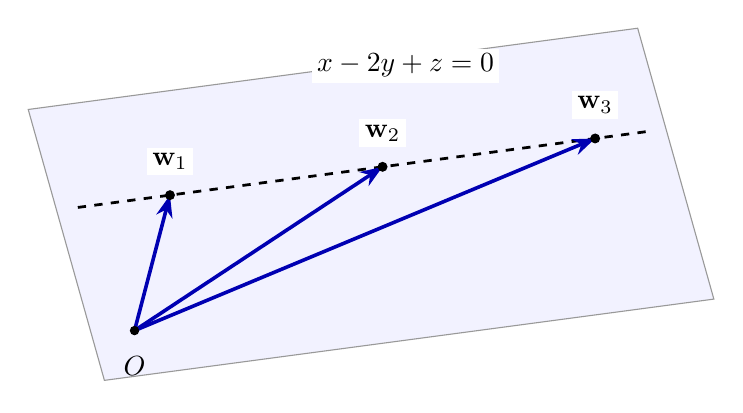
\begin{tikzpicture}[x={(.9cm,.12cm)},y={(-.45cm,1.6cm)}]

\draw[fill=blue!5,draw=black!40] (-.6,-.35)--(8,-.35)--(8,1.8)--(-.6,1.8)--cycle;
\draw[black,dashed,line width=1pt] (-.3,1)--(7.8,1);
\coordinate (O) at (0,0);
\coordinate (Wone) at (1,1);
\coordinate (Wtwo) at (4,1);
\coordinate (Wthree) at (7,1);
\draw[vec] (O)--(Wone);
\draw[vec] (O)--(Wtwo);
\draw[vec] (O)--(Wthree);
\fill (O) circle (1.7pt);
\node[below=6pt] at (O) {$O$};
\foreach \p in {Wone,Wtwo,Wthree} {\fill (\p) circle (1.8pt);}
\node[lab,above=7pt] at (Wone) {$\mathbf w_1$};
\node[lab,above=7pt] at (Wtwo) {$\mathbf w_2$};
\node[lab,above=7pt] at (Wthree) {$\mathbf w_3$};
\node[lab] at (4.7,1.75) {$x-2y+z=0$};
\end{tikzpicture}
\end{document}
